\documentclass[lettersize,journal]{IEEEtran}

\usepackage{amsmath,amsfonts,amssymb}
\usepackage{algorithmic}
\usepackage{algorithm}
\usepackage{array}
\usepackage{booktabs}
\usepackage{multirow}
\usepackage{subcaption}
\usepackage{stfloats}
\usepackage{url}
\usepackage{graphicx}
\usepackage{cite}
\usepackage{balance}
\usepackage{microtype}
\usepackage{bm}

% Float Capacity & Layout Optimization for Exact 10-Page Fit
\setcounter{topnumber}{4}
\setcounter{bottomnumber}{4}
\setcounter{totalnumber}{6}
\setcounter{dbltopnumber}{3}

\renewcommand{\topfraction}{0.95}
\renewcommand{\bottomfraction}{0.95}
\renewcommand{\textfraction}{0.05}
\renewcommand{\floatpagefraction}{0.85}
\renewcommand{\dbltopfraction}{0.95}
\renewcommand{\dblfloatpagefraction}{0.85}

\setlength{\textfloatsep}{5pt plus 1pt minus 1pt}
\setlength{\floatsep}{4pt plus 1pt minus 1pt}
\setlength{\dbltextfloatsep}{6pt plus 1pt minus 1pt}
\setlength{\dblfloatsep}{4pt plus 1pt minus 1pt}

\graphicspath{{figs/}{fig/}{../figs/}{../fig/}}

\hyphenation{op-tical net-works semi-conduc-tor IEEE-Xplore micro-controller MicroPhys-BMS}

\begin{document}
	
	\title{Physics-Informed Knowledge Distillation for Real-Time State-of-Charge Estimation of $\text{LiFePO}_4$ Batteries on Automotive Microcontrollers}

\author{Hamid~Daneshvar,~\IEEEmembership{Student~Member,~IEEE,}
	and~Masoud~Masih-Tehrani,~\IEEEmembership{Member,~IEEE}%
	\thanks{Manuscript received August 20, 2026. This work was supported in part by the Vehicle, Fuel, and Environment Research Institute (VFERI) and the School of Automotive Engineering at Iran University of Science and Technology (IUST). \textit{(Corresponding author: Masoud Masih-Tehrani.)}}%
	\thanks{Hamid Daneshvar and Masoud Masih-Tehrani are with the School of Automotive Engineering, Iran University of Science and Technology (IUST), Tehran 16846-13114, Iran (e-mail: hamid\_daneshvar@auto.iust.ac.ir; masih@iust.ac.ir).}}

\markboth{IEEE Transactions on Transportation Electrification,~Vol.~XX, No.~XX,~August~2026}%
{Daneshvar and Masih-Tehrani: Physics-Informed Knowledge Distillation for Real-Time SOC Estimation}

\maketitle

\begin{abstract}
	Precise state-of-charge (SOC) estimation in Lithium Iron Phosphate ($\text{LiFePO}_4$ or LFP) batteries remains an enduring industrial challenge for automotive battery management systems (BMS) due to the ultra-flat open-circuit voltage (OCV) plateau ($\text{d}V_{\text{ocv}}/\text{d}\text{SOC} \approx 0.1\text{--}0.5\text{ mV/\%}$) and protracted non-linear solid-phase relaxation dynamics. While heavy data-driven ensembles and electrochemical partial differential equation (PDE) solvers capture these path-dependent transitions, their computational complexity and excessive memory footprints prohibit deterministic real-time execution on resource-constrained automotive microcontrollers. In this study, we propose \textit{MicroPhys-BMS}, an end-to-end Physics-Informed Machine Learning Knowledge Distillation (PIML-KD) framework that compresses complex non-linear electro-thermal relaxation dynamics into an ultra-compact student Micro-MLP architecture ($12 \to 32 \to 16 \to 1$, 961 parameters) for ISO 26262 ASIL-D compliant microcontrollers. The framework extracts a 12-dimensional domain-guided physical feature vector encoding Arrhenius reaction kinetics, dynamic ohmic overpotential, logarithmic solid-phase diffusion scaling, and differential relaxation gradients. A 300-tree gradient-boosted decision tree (LightGBM) teacher supervises the student network via a composite physics-calibrated objective combining adaptive Huber distillation, task-level mean squared error, and quadratic physical boundary constraints enforcing $\text{SOC} \in [0.0, 1.0]$. Validated against extensive Stanford LFP operational telemetry, the proposed student Micro-MLP achieves a nominal $25^\circ\text{C}$ case-split MAE of 0.454\% and RMSE of 1.236\% ($R^2 = 0.9986$), outperforming the LightGBM teacher (MAE = 0.488\%). Under unseen cell generalization tests, the model records SOC MAEs of 2.48\% on cell YX07 and 3.35\% on cell YX08, reducing estimation errors by 42.3\% and 22.1\% relative to the Stanford baseline benchmark target (4.30\%). For short-term rest horizons, the framework enables robust Coulomb counting re-initialization at 30~s (MAE = 1.170\%) and converges to 0.339\% at 300~s. Furthermore, the model demonstrates high resilience against analog front-end (AFE) voltage noise (MAE = 1.336\% under $\pm 5.0\text{ mV}$ perturbation) and multi-temperature shifts (MAE = 2.689\% at 35$^\circ$C), with 95.94\% of cumulative error distribution remaining within $\le 2.0\%$. Synthesized into a MISRA-C:2012 compliant static C header without dynamic heap allocation (\texttt{malloc}), the deployed model requires only 3.75~kB Flash, 192~Bytes SRAM, and an execution latency of $\approx 12\ \mu\text{s}$ on an ARM Cortex-M4 at 160~MHz, achieving over 99.7\% memory compression compared to standard tree ensembles.
\end{abstract}

\begin{IEEEkeywords}
	Automotive microcontrollers, battery management system (BMS), knowledge distillation (KD), lithium iron phosphate (LFP) battery, physics-informed machine learning (PIML), state-of-charge (SOC).
\end{IEEEkeywords}
	\section*{Nomenclature}
\addcontentsline{toc}{section}{Nomenclature}

\noindent
{\scriptsize
	\renewcommand{\arraystretch}{0.78}
	\begin{tabular}{@{}p{1.15cm}p{5.75cm}@{}}
		\toprule
		\multicolumn{2}{@{}l}{\textbf{Variables and Physical Descriptors}} \\
		\midrule
		$t, V_{\text{mea}}, V_{10}$ & Rest time (s), measured voltage, $V$ at $t=10$ s (V). \\
		$\text{SOC}_{\text{mea}}, y_{\text{std}}$ & Coulomb-counted SOC, predicted student SOC. \\
		$I_m, R, I_{\text{flag}}$ & Pre-rest current (A), dynamic resistance ($\Omega$), direction ($\pm 1$). \\
		$T_{\text{env}}, \Delta T$ & Ambient temperature and thermal gradient ($^\circ$C). \\
		$\Delta V_{10}$ & Relaxation overpotential gradient, $V_{\text{mea}}(t) - V_{10}$. \\
		$\tau_{\text{log}}, P_{\text{ohm}}$ & Diffusion scale $\ln(t+1)$; ohmic dissipation $R \cdot I_m$. \\
		$\Phi_{\text{Arr}}$ & Arrhenius factor $\exp(-E_a/(R_g T_K))$; $E_a = 35.0$ kJ/mol. \\
		$X_{\text{raw}}, X_{\text{PIML}}$ & Raw 9-D and physics-informed 12-D feature vectors. \\
		$y_{\text{true}}, y_{\text{teach}}$ & Ground-truth SOC and teacher soft targets. \\
		$\mathcal{L}_{\text{PIMD}}$ & Composite physics-informed distillation loss. \\
		$\alpha, \beta, \lambda_{\text{mse}}, \lambda_{\text{bounds}}$ & Loss weights ($0.40, 0.015, 0.50, 0.02$). \\
		$\mathbf{W}_l, \mathbf{b}_l, \sigma_{\text{SiLU}}$ & Layer $l$ weights/biases; SiLU $x/(1+e^{-x})$. \\
		$T_{\text{exec}}, M_{\text{Flash}}, M_{\text{SRAM}}$ & Latency ($\mu$s), Flash and SRAM footprints. \\
		\midrule
		\multicolumn{2}{@{}l}{\textbf{Acronyms and Abbreviations}} \\
		\midrule
		AFE, ASIL-D & Analog Front-End; Automotive Safety Integrity Level D (ISO 26262). \\
		BMS, VCU & Battery Management System; Vehicle Control Unit. \\
		ECM, EKF, GBDT & Equivalent Circuit Model; Extended Kalman Filter; Gradient Boosted Decision Tree. \\
		LFP, OCV, PIML & Lithium Iron Phosphate; Open-Circuit Voltage; Physics-Informed Machine Learning. \\
		MAE, RMSE, WCET & Mean Absolute Error; Root-Mean-Square Error; Worst-Case Execution Time. \\
		MISRA-C & Motor Industry Software Reliability Association (2012). \\
		\bottomrule
	\end{tabular}
}
	\begin{figure*}[!t]
	\centering
	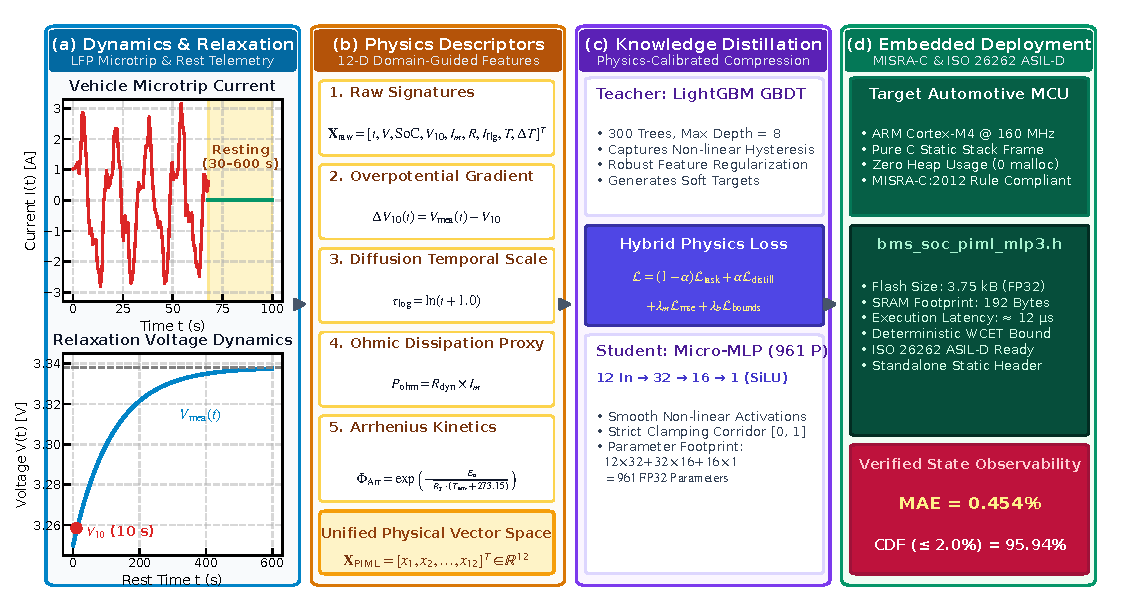
\includegraphics[width=7.0in]{Fig1_PIML_KD_Framework_V2-1_2.pdf}
	\caption{Architectural overview of the proposed \textit{MicroPhys-BMS} framework. (a) Real-world operational vehicle microtrip current profile and transient relaxation voltage dynamics ($30\text{--}600\text{ s}$). (b) Domain-guided physical feature engineering extracting 12-dimensional electro-thermal descriptors ($X_{\text{PIML}}$). (c) Hybrid knowledge distillation compressing a 300-tree LightGBM ensemble into a 961-parameter student Micro-MLP under multi-objective physics-calibrated loss. (d) Automotive embedded deployment pipeline yielding a MISRA-C compliant, zero-\texttt{malloc} static C header (\texttt{bms\_soc\_piml\_mlp3.h}) for deterministic execution on automotive microcontrollers.}
	\label{fig:framework_overview}
\end{figure*}

\section{Introduction}
\label{sec:introduction}

\IEEEPARstart{L}{ithium-ion} batteries, particularly Lithium Iron Phosphate ($\text{LiFePO}_4$ or LFP), have established decisive dominance as the preferred electrochemical energy storage technology for commercial electric vehicles (EVs), urban transit buses, and heavy-duty grid energy storage systems \cite{masih2013optimum, rahimirad2019battery, attia2020closed, rout2024online}.

\subsection{Industrial Context and the LFP Flat-Plateau Challenge}
\label{sec:intro_a}

Driven by their exceptional inherent thermal runaway resilience, operational cycle life exceeding 3000 full equivalent cycles, non-toxic cobalt- and nickel-free chemistry, and superior raw material cost-effectiveness, LFP battery packs have achieved dominant market penetration in commercial transportation electrification \cite{masih2013optimum, rahimirad2019battery, attia2020closed, severson2019data, najafi2025adaptive}. Despite these compelling safety and economic advantages, deploying LFP battery chemistries in advanced automotive battery management systems (BMS) introduces severe, non-linear state observation challenges that are fundamentally distinct from nickel-manganese-cobalt (NMC) or lithium titanate (LTO) chemistries \cite{roscher2011dynamic, hu2012comparative, sorouri2025breaking, wang2025lifepo4}.

The central impediment to reliable on-board state-of-charge (SOC) tracking in LFP cells resides in the thermodynamic flat open-circuit voltage (OCV) plateau, which spans an extensive operational corridor from approximately $20\%$ to $80\%$ SOC \cite{sorouri2025breaking, xiong2018towards}. From a solid-state electrochemical perspective, lithium deintercalation and insertion in the olivine $\text{LiFePO}_4$ lattice proceed via a first-order phase transformation between two distinct ordered crystal phases: the fully lithiated triphylite ($\text{LiFePO}_4$) phase and the fully delithiated heterosite ($\text{FePO}_4$) phase \cite{sorouri2025breaking}. In the thermodynamic miscibility gap, the chemical potential of lithium ions $\mu_{\text{Li}^+}$ remains strictly constant across the phase boundary. According to the Nernst-Planck thermodynamic relation:
\begin{equation}
	\label{eq:nernst_ocv}
	V_{\text{ocv}}(\text{SOC}, T_K) = -\frac{\mu_{\text{Li}^+}^{\text{cathode}}(\text{SOC}, T_K) - \mu_{\text{Li}^+}^{\text{anode}}(\text{SOC}, T_K)}{F},
\end{equation}
where $F = 96485.33\ \text{C/mol}$ denotes Faraday's constant and $T_K$ is absolute temperature. Consequently, as illustrated in Fig.~\ref{fig:physical_motivation}(a), the incremental derivative of the equilibrium open-circuit voltage with respect to SOC is virtually zero throughout this wide domain:
\begin{equation}
	\label{eq:flat_plateau_derivative}
	\left. \frac{\partial V_{\text{ocv}}(\text{SOC}, T_K)}{\partial \text{SOC}} \right|_{\text{SOC} \in [0.20, 0.80]} \approx 0.10 \text{--} 0.50\ \text{mV/\%}.
\end{equation}

\begin{figure}[!t]
	\centering
	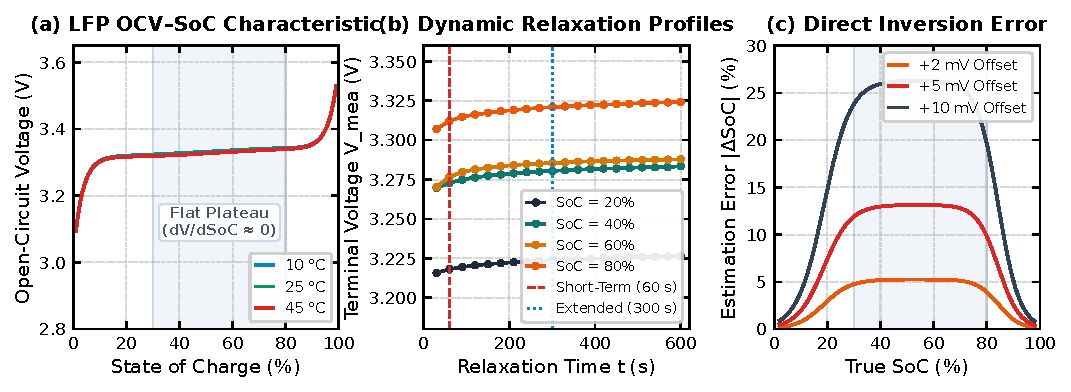
\includegraphics[width=\columnwidth]{Figure_2_Physical_Motivation_Final_IEEE_2.pdf}
	\caption{Electrochemical characteristics and observability dilemma of LFP cells. (a) Static $V_{\text{ocv}}$--SOC characteristic across $10^\circ\text{C}$, $25^\circ\text{C}$, and $45^\circ\text{C}$ highlighting the flat plateau. (b) Dynamic terminal voltage relaxation trajectories across varied SOC levels ($20\%$, $40\%$, $60\%$, and $80\%$). (c) Direct thermodynamic inversion error under typical analog front-end (AFE) sensing offsets ($+2\text{ mV}$, $+5\text{ mV}$, and $+10\text{ mV}$).}
	\label{fig:physical_motivation}
\end{figure}

Compounding this flat derivative is significant path-dependent electrochemical hysteresis between charging and discharging branches, which arises from mechanical coherency strain energy and phase-boundary interfacial resistance \cite{roscher2011dynamic, sorouri2025breaking}. Because the static voltage curve is nearly horizontal, any direct numerical inversion of the measured terminal voltage $V_{\text{mea}}$ to deduce battery state exhibits extreme mathematical ill-conditioning. As demonstrated in Fig.~\ref{fig:physical_motivation}(c), an analog front-end (AFE) measurement offset of merely $+5.0\ \text{mV}$ induces catastrophic SOC estimation errors exceeding $20\%\text{--}30\%$ across the plateau domain.

Furthermore, dynamic vehicle operation introduces prolonged, non-linear voltage relaxation tails following current pulses (Fig.~\ref{fig:physical_motivation}(b)). Following current cessation during real-world vehicle microtrips (such as regenerative braking events or urban traffic stops), the terminal voltage does not instantaneously recover to thermodynamic equilibrium $V_{\text{ocv}}$. Instead, it undergoes a complex, multi-time-scale relaxation process governed by fast double-layer capacitive discharge ($\tau_1 \le 10\ \text{s}$) and sluggish solid-state lithium-ion diffusion within the porous active electrode particles ($\tau_2 \ge 100\ \text{s}$), lasting up to several hours \cite{che2025enhanced, sorouri2025breaking}.

In commercial automotive BMS applications, short rest intervals ($30\ \text{s}$ to $600\ \text{s}$) represent crucial operational opportunities for re-initializing and resetting the cumulative integration drift inherent to Coulomb counting algorithms \cite{waag2014critical, che2025enhanced}. However, sampling the terminal voltage prematurely during non-equilibrium relaxation windows without accurately back-extrapolating the true equilibrium overpotential introduces large state initialization errors. Developing a computationally deterministic and mathematically bounded algorithm capable of extracting equilibrium signatures from short-term relaxation telemetry is therefore vital for next-generation transportation electrification.

\subsection{Limitations of Classical Observers and Heavy Tree Ensembles}
\label{sec:intro_b}

To track battery state dynamics under operational driving loads, conventional automotive BMS architectures deploy state estimation algorithms falling into two broad paradigms: equivalent circuit model (ECM)-based adaptive observers and data-driven machine learning models \cite{masih2018novel, waag2014critical, najafi2024statepower, xu2025state}.

Classical state observation frameworks rely heavily on Extended Kalman Filters (EKF), Unscented Kalman Filters (UKF), Adaptive Extended Kalman Filters (AEKF), or recursive least squares (RLS) coupled with low-order RC equivalent circuits \cite{plett2004extended, xiong2018towards, wei2022future, hou2026online, fan2025state}. In these recursive formulations, the state correction step is strictly driven by the voltage innovation residual $\tilde{y}_k = V_{\text{mea},k} - \hat{V}_{t,k}$, weighted through the Kalman gain matrix $\mathbf{K}_k$ \cite{plett2004extended, wei2022future}:
Classical state observation frameworks rely on Extended Kalman Filters (EKF), Unscented Kalman Filters (UKF), Adaptive EKF, or recursive least squares (RLS) coupled with low-order RC equivalent circuits \cite{plett2004extended, xiong2018towards, wei2022future, hou2026online, fan2025state}. The state correction step uses the voltage innovation residual weighted through the Kalman gain $\mathbf{K}_k = \mathbf{P}_{k|k-1}\mathbf{H}_k^T(\mathbf{H}_k\mathbf{P}_{k|k-1}\mathbf{H}_k^T + \mathbf{R}_v)^{-1}$, where $\mathbf{H}_k = \partial V_{\text{ocv}}/\partial \text{SOC}$ is the observation Jacobian. Within the LFP flat plateau ($\text{SOC} \in [0.20, 0.80]$), $\mathbf{H}_k \to \mathbf{0}$, causing $\mathbf{K}_k \to \mathbf{0}$ \cite{wei2022future, sorouri2025breaking}. Feedback correction collapses into open-loop Coulomb counting $\text{SOC}_k = \text{SOC}_{k-1} - (\eta_c \Delta t / Q_{\text{nom}})(I_k + \delta I_k)$, where $\delta I_k$ captures sensor bias and ADC quantization errors; accumulated state error grows unbounded over multi-hour cycles \cite{waag2014critical, rout2024online, dong2026secure}.

While high-fidelity electrochemical physics-based models capture solid-phase diffusion and Butler-Volmer kinetics with high fidelity, their non-linear partial differential algebraic equation (PDAE) structure incurs prohibitive computational complexity \cite{sorouri2025breaking, che2025enhanced, sorouri2026physics}. Solving coupled PDAE systems exceeds the deterministic execution budgets and static memory allocations of standard automotive microcontrollers (e.g., ARM Cortex-M4, Infineon AURIX TC3xx, and NXP S32K) by multiple orders of magnitude \cite{yahyaei2023embedded}.

To overcome physical modeling bottlenecks, recent benchmark studies, most notably the 2025 Stanford relaxation methodology \cite{che2025enhanced}, introduced multi-stage data-driven pipelines utilizing decision tree ensembles (such as sequential 3-stage Random Forests) to capture non-linear relaxation voltage tails during vehicle rest periods. Although tree ensembles improve state tracking across flat OCV intervals, their algorithmic complexity presents severe deployment barriers in production automotive environments \cite{lin2020mcunet, cui2025toward}.

As quantified in Section~\ref{sec:res_g}, the reference Stanford 3-stage Random Forest (RF) baseline \cite{che2025enhanced} requires approximately $1420.0\ \text{kB}$ of Flash memory and contains $\approx 60,000$ parameters. Traversing deep ensemble decision paths induces an inference latency of $1850.0\ \mu\text{s}$ ($1.85\ \text{ms}$) on a standard ARM Cortex-M4 core at 160~MHz. Similarly, sequence-based deep models such as Tabular Transformers ($142.0\ \text{kB}$ Flash, $35.5\text{k}$ parameters) \cite{chen2024transformer} and Vanilla LSTM networks ($53.0\ \text{kB}$ Flash, $13.2\text{k}$ parameters) \cite{xiong2018towards} violate the stringent static memory allocations ($M_{\text{Flash}} \le 16\ \text{kB}$) and worst-case execution time budgets ($T_{\text{exec}} \le 50\ \mu\text{s}$) of commercial BMS electronic control units (ECUs). Furthermore, tree ensembles with irregular branching structures and unconstrained recurrent networks cannot provide static execution determinism, preventing ISO 26262 ASIL-D functional safety certification \cite{yahyaei2023embedded}.

\subsection{Proposed Physics-Informed Knowledge Distillation Paradigm}
\label{sec:intro_c}

To resolve the fundamental trade-off between non-linear representational capacity and embedded execution determinism, Physics-Informed Machine Learning coupled with Knowledge Distillation (PIML-KD) offers an effective paradigm \cite{karniadakis2021physics, li2026condition, amirkhani2021robust, liu2024unsupervised}. Under this architecture, the state estimation problem is decoupled into an offline high-capacity teacher learning stage and an on-chip, physics-constrained student execution engine \cite{amirkhani2021robust, najafi2024statepower, li2026condition}.

As conceptualized in Fig.~\ref{fig:framework_overview}, the teacher model comprises an offline Gradient Boosted Decision Tree (LightGBM) ensemble parameterized with 300 estimators \cite{ke2017lightgbm}. This teacher possesses sufficient non-linear depth to internalize complex, path-dependent electrochemical hysteresis, state-dependent solid-phase diffusion delays, and multi-regime relaxation profiles across the complete operating space without run-time execution limits.

To transfer this non-linear mapping capability into an ultra-efficient edge format, we construct a compact student Multilayer Perceptron (Micro-MLP) featuring a $12 \to 32 \to 16 \to 1$ topology ($961$ total parameters) \cite{lin2020mcunet}. Rather than treating distillation as an unconstrained empirical curve-fitting problem, the student network is strictly regularized via domain-guided physical laws \cite{karniadakis2021physics, sorouri2026physics}: (i) differential relaxation overpotentials ($\Delta V_{10} = V_{\text{mea}}(t) - V_{10}$), (ii) logarithmic diffusion scales ($\tau_{\text{log}} = \ln(t + 1.0)$), (iii) dynamic ohmic dissipation ($P_{\text{ohm}} = R \cdot I_m$), (iv) Arrhenius reaction kinetics ($\Phi_{\text{Arr}} = \exp(-E_a/(R_g T_K))$ with $E_a = 35.0\ \text{kJ/mol}$) \cite{rahimirad2019battery, meng2025domain}, and (v) a composite distillation loss combining Smooth-$L_1$ Huber loss and quadratic physical boundary penalties enforcing $\text{SOC} \in [0.0, 1.0]$. The framework synthesizes directly into a zero-\texttt{malloc} static C header for deterministic execution on automotive electronic control units \cite{yahyaei2023embedded}.

\subsection{Core Contributions and Article Organization}
\label{sec:intro_d}

The principal contributions of this work are summarized as follows:
\begin{enumerate}
	\item \textbf{Physics-Informed Domain-Guided 12-D Feature Engineering:} Formulating a 12-dimensional physical input representation ($X_{\text{PIML}}$) that augments raw sensor telemetry with differential overpotentials ($\Delta V_{10}$), logarithmic diffusion scaling ($\tau_{\text{log}}$), dynamic ohmic dissipation ($P_{\text{ohm}}$), and Arrhenius reaction kinetics ($\Phi_{\text{Arr}}$ with $E_a = 35.0\ \text{kJ/mol}$) \cite{rahimirad2019battery, li2026condition}.
	\item \textbf{Physically Calibrated Hybrid Knowledge Distillation:} Developing a teacher--student compression pipeline wherein a 300-tree LightGBM teacher supervises an ultra-lightweight student Micro-MLP ($12 \to 32 \to 16 \to 1$, $961$ total parameters) under a multi-objective loss enforcing thermodynamic boundary validity \cite{ke2017lightgbm, amirkhani2021robust}.
	\item \textbf{Multi-Regime Generalization and Telemetry Noise Robustness:} Achieving a nominal $25^\circ\text{C}$ MAE of $0.454\%$ and RMSE of $1.236\%$ ($R^2 = 0.9986$). On unseen cells YX07 and YX08, the model achieves MAEs of $2.48\%$ and $3.35\%$, beating the Stanford target ($4.30\%$) \cite{che2025enhanced} by $42.3\%$ and $22.1\%$. The framework enables Coulomb counting resets at $30\ \text{s}$ ($\text{MAE} = 1.170\%$, converging to $0.339\%$ at $300\ \text{s}$) and resists $\pm 5.0\ \text{mV}$ AFE noise ($\text{MAE} = 1.336\%$).
	\item \textbf{MISRA-C Compliant Static Deployment Pipeline:} Providing an automated synthesis pipeline exporting the student Micro-MLP into a static C header (\texttt{bms\_soc\_piml\_mlp3.h}) requiring only $3.75\ \text{kB}$ Flash, $192\ \text{Bytes}$ SRAM, and $12.0\ \mu\text{s}$ latency on an ARM Cortex-M4 at $160\ \text{MHz}$ \cite{yahyaei2023embedded, lin2020mcunet}.
\end{enumerate}

The remainder of this article is structured as follows: Section~\ref{sec:methodology} details the mathematical formulation of the 12 PIML descriptors, teacher pipeline, distillation loss, and static C generation. Section~\ref{sec:results} presents comprehensive experimental results. Section~\ref{sec:conclusion} concludes the article.
	\section{Methodology}
\label{sec:methodology}

\subsection{Physics-Informed Feature Engineering and Relaxation Dynamics}
\label{sec:meth_a}

Accurate observation of LFP cell state during transient vehicle stops requires capturing multi-time-scale relaxation kinetics \cite{sorouri2025breaking, xiong2018towards}. In production BMS, real-time measurements are limited to voltage, current, and temperature \cite{waag2014critical, lin2020mcunet}. To establish an electrochemically meaningful input without PDAE solver overhead, the proposed framework transforms raw 9-D telemetry $X_{\text{raw}} \in \mathbb{R}^9$ into 12-D physics-informed descriptors $X_{\text{PIML}} \in \mathbb{R}^{12}$.

\subsubsection{Two-Phase Coexistence and Electrochemical Kinetics}
In Lithium Iron Phosphate cathode materials, intercalation and deintercalation proceed via a first-order phase transformation between two distinct ordered crystal phases: the lithium-rich triphylite ($\text{LiFePO}_4$) and lithium-poor heterosite ($\text{FePO}_4$) phases. The open-circuit equilibrium potential $V_{\text{ocv}}$ is governed by the difference in chemical potentials between the positive and negative active particles:
\begin{equation}
	\label{eq:chemical_potential}
	V_{\text{ocv}}(\text{SOC}, T_K) = -\frac{\mu_{\text{cathode}}(\text{SOC}, T_K) - \mu_{\text{anode}}(\text{SOC}, T_K)}{F},
\end{equation}
where $F = 96485.33\ \text{C/mol}$ is Faraday's constant. Across the extensive two-phase coexistence region ($0.20 \le \text{SOC} \le 0.80$), the active phase boundary propagates at nearly constant chemical potential ($\mu_{\text{LiFePO}_4} - \mu_{\text{FePO}_4} = \text{const}$), yielding the characteristic flat plateau with $\text{d}V_{\text{ocv}}/\text{d}\text{SOC} \approx 0.10\text{--}0.50\ \text{mV/\%}$.

\subsubsection{Raw Telemetry Measurement Space}
The raw telemetry vector $X_{\text{raw}}$ encapsulates real-time operational and resting signals recorded at sample tick $t$:
\begin{equation}
	\label{eq:raw_feature_vector}
	X_{\text{raw}} = \left[ t, V_{\text{mea}}, \text{SOC}_{\text{mea}}, V_{10}, I_m, R, I_{\text{flag}}, T_{\text{env}}, \Delta T \right]^T,
\end{equation}
where $t$ represents the elapsed resting duration ($30\ \text{s} \le t \le 600\ \text{s}$), $V_{\text{mea}}$ is the measured terminal voltage at time $t$, $\text{SOC}_{\text{mea}}$ denotes the uncorrected preliminary SOC obtained via Coulomb counting integration from the preceding microtrip, $V_{10}$ is the reference terminal voltage recorded at $t = 10\ \text{s}$, $I_m$ is the moving-average pulse current prior to rest cessation, $R$ is the dynamic internal cell resistance, $I_{\text{flag}} \in \{-1, +1\}$ denotes the current direction indicator ($-1$ for charge, $+1$ for discharge), $T_{\text{env}}$ is the ambient environmental temperature ($^\circ\text{C}$), and $\Delta T = T_{\text{cell}} - T_{\text{env}}$ is the surface-to-ambient thermal gradient.

\subsubsection{Electrochemical Derivations of Physical Descriptors}
Directly feeding raw telemetry $X_{\text{raw}}$ into conventional neural estimators results in poor cross-cell and multi-temperature generalization due to unmodeled non-linear phase-boundary propagation and concentration polarization delays \cite{sorouri2025breaking, wang2025lifepo4}. To capture the underlying electrochemistry, four domain-guided transformations are derived:

\begin{enumerate}
	\item \textbf{Differential Relaxation Overpotential Gradient ($\Delta V_{10}$):}
	Following load current interruption, the instantaneous terminal voltage $V(t)$ is governed by the superposition of equilibrium potential $V_{\text{ocv}}$, instantaneous ohmic drop $I R_0$, solid-electrolyte interphase (SEI) charge-transfer overpotentials $\eta_{\text{ct}}(t)$, and solid-phase diffusion overpotentials $\eta_{\text{diff}}(t)$:
	\begin{equation}
		\label{eq:voltage_decomposition}
		V(t) = V_{\text{ocv}}(\text{SOC}, T_K) \pm I R_0 \pm \eta_{\text{ct}}(t) \pm \eta_{\text{diff}}(t) + \delta v_{\text{dc}},
	\end{equation}
	where $\delta v_{\text{dc}}$ represents sensor calibration offset. Because the ohmic drop collapses instantaneously ($t < 1\ \text{ms}$) and the double-layer capacitance $C_{\text{dl}}$ discharges rapidly ($\tau_{\text{dl}} \approx R_{\text{ct}} C_{\text{dl}} \le 10\ \text{s}$), the voltage at $t = 10\ \text{s}$ serves as a physical boundary anchor isolating pure solid-phase diffusion:
	\begin{equation}
		\label{eq:v10_anchor}
		V_{10} \approx V_{\text{ocv}}(\text{SOC}, T_K) \pm \eta_{\text{diff}}(10\ \text{s}) + \delta v_{\text{dc}}.
	\end{equation}
	Defining the differential overpotential gradient as:
	\begin{equation}
		\label{eq:delta_v10}
		\Delta V_{10}(t) = V_{\text{mea}}(t) - V_{10} = \eta_{\text{diff}}(t) - \eta_{\text{diff}}(10\ \text{s}),
	\end{equation}
	the common-mode sensor DC offset $\delta v_{\text{dc}}$ and the ohmic step $I R_0$ are completely eliminated by algebraic cancellation, yielding a clean overpotential recovery signature invariant to sensor calibration drift.
	
	\item \textbf{Logarithmic Diffusion Relaxation Time Scale ($\tau_{\text{log}}$):}
	Solid-phase lithium transport within spherical active electrode particles of radius $R_p$ is governed by Fick's second law of diffusion in spherical coordinates:
	\begin{equation}
		\label{eq:fick_diffusion}
		\frac{\partial c_s(r, t)}{\partial t} = D_s \left( \frac{\partial^2 c_s(r, t)}{\partial r^2} + \frac{2}{r} \frac{\partial c_s(r, t)}{\partial r} \right),
	\end{equation}
	where $c_s(r, t)$ is solid lithium concentration and $D_s$ is solid-phase diffusion coefficient. According to Crank's analytical series solution, the volumetric mean concentration $\bar{c}_s(t)$ approaches surface equilibrium as $1 - (6/\pi^2)\sum_{n=1}^{\infty} n^{-2} \exp(-n^2 \pi^2 D_s t / R_p^2)$. For $t \ge 30\ \text{s}$, the leading exponential dominates, yielding logarithmic decay $\eta_{\text{diff}}(t) \propto \ln(t / \tau_{\text{diff}})$. To linearize this across $t \in [30, 600]\ \text{s}$, the logarithmic diffusion scale is $\tau_{\text{log}}(t) = \ln(t + 1.0)$, providing a linearized diffusion coordinate. This compresses the dynamic range of the temporal domain and provides the neural estimator with a linearized diffusion coordinate.
	
	\item \textbf{Dynamic Ohmic Polarization Dissipation ($P_{\text{ohm}}$):}
	The magnitude of non-equilibrium concentration polarization generated during the active microtrip is directly proportional to the product of dynamic internal impedance and load current excitation:
	\begin{equation}
		\label{eq:p_ohm}
		P_{\text{ohm}} = R \cdot I_m,
	\end{equation}
	which acts as a proxy for the total Joule dissipation and overpotential accumulation incurred prior to current cessation.
	
	\item \textbf{Arrhenius Electrochemical Kinetics Factor ($\Phi_{\text{Arr}}$):}
	Charge-transfer resistance and solid-state lithium diffusivity are strongly temperature-dependent, governed by the Butler-Volmer exchange current density $i_0(T_K)$ and Arrhenius reaction rate law:
	\begin{equation}
		\label{eq:arrhenius_derivation}
		i_0(T_K) = i_{0,\text{ref}} \exp\left( -\frac{E_a}{R_g} \left( \frac{1}{T_K} - \frac{1}{T_{\text{ref}}} \right) \right),
	\end{equation}
	where $E_a = 35.0\ \text{kJ/mol}$ ($35000.0\ \text{J/mol}$) is the fundamental activation energy barrier for lithium deintercalation in olivine $\text{LiFePO}_4$ cathodes, $R_g = 8.314\ \text{J/(mol}\cdot\text{K)}$ is the universal gas constant, and $T_K = T_{\text{env}} + 273.15$ is absolute temperature in Kelvin \cite{rahimirad2019battery, li2026condition}. To embed thermodynamic consistency across wide operational thermal envelopes (ranging from sub-zero to elevated regimes), the Arrhenius descriptor is formulated as:
	\begin{equation}
		\label{eq:arrhenius_kinetics}
		\Phi_{\text{Arr}} = \exp\left( -\frac{E_a}{R_g \cdot (T_{\text{env}} + 273.15)} \right).
	\end{equation}
\end{enumerate}

\begin{table}[!t]
	\caption{Formulation and Significance of the 12 PIML Descriptors ($X_{\text{PIML}}$)}
	\label{tab:piml_features}
	\centering
	\resizebox{\columnwidth}{!}{%
		\begin{tabular}{cclp{3.8cm}}
			\toprule
			\textbf{Index} & \textbf{Symbol} & \textbf{Mathematical Definition} & \textbf{Physical / Electrochemical Domain} \\
			\midrule
			$x_1$ & $t$ & Sample tick & Elapsed resting duration ($30\text{--}600\text{ s}$) \\
			$x_2$ & $V_{\text{mea}}$ & Terminal voltage $V(t)$ & Macroscopic electrical potential \\
			$x_3$ & $\text{SOC}_{\text{mea}}$ & $\int I \text{d}t / Q_{\text{nom}}$ & Coulomb counting preliminary state \\
			$x_4$ & $V_{10}$ & $V(t=10\text{ s})$ & Fast double-layer polarization anchor \\
			$x_5$ & $I_m$ & Pre-rest mean current & Pre-rest dynamic load excitation \\
			$x_6$ & $R$ & Dynamic resistance $\Delta V / \Delta I$ & Solid-electrolyte interphase impedance \\
			$x_7$ & $I_{\text{flag}}$ & $\text{sgn}(I_m) \in \{-1, +1\}$ & Charge/discharge directional hysteresis \\
			$x_8$ & $\Phi_{\text{Arr}}$ & $\exp\left(-\frac{E_a}{R_g T_K}\right)$ & Arrhenius reaction kinetics factor \\
			$x_9$ & $\Delta T$ & $T_{\text{cell}} - T_{\text{env}}$ & Internal-to-ambient thermal differential \\
			$x_{10}$ & $\Delta V_{10}$ & $V_{\text{mea}}(t) - V_{10}$ & Solid-phase diffusion overpotential \\
			$x_{11}$ & $\tau_{\text{log}}$ & $\ln(t + 1.0)$ & Fickian diffusion logarithmic time scale \\
			$x_{12}$ & $P_{\text{ohm}}$ & $R \cdot I_m$ & Dynamic ohmic polarization dissipation \\
			\bottomrule
		\end{tabular}%
	}
\end{table}

The resulting 12-dimensional physical descriptor vector is represented compactly in two lines to preserve strict column alignment:
\begin{equation}
	\label{eq:piml_vector}
	\begin{aligned}
		X_{\text{PIML}} = \big[ & t, V_{\text{mea}}, \text{SOC}_{\text{mea}}, V_{10}, I_m, R, \\
		& I_{\text{flag}}, \Phi_{\text{Arr}}, \Delta T, \Delta V_{10}, \tau_{\text{log}}, P_{\text{ohm}} \big]^T.
	\end{aligned}
\end{equation}
Prior to model training and inference, each feature dimension $x_j$ is standardized using immutable compile-time mean $\mu_j$ and scale $\sigma_j$ parameters:
\begin{equation}
	\label{eq:feature_standardization}
	\tilde{x}_j = \frac{x_j - \mu_j}{\sigma_j}, \quad j = 1, \dots, 12.
\end{equation}

\subsection{Offline High-Capacity Teacher Model Architecture}
\label{sec:meth_b}

To effectively capture the complex, multi-dimensional regression surface governing electrochemical hysteresis and diffusion recovery without run-time computational constraints, an offline high-capacity teacher model is constructed using a Gradient Boosted Decision Tree (GBDT) ensemble via LightGBM \cite{ke2017lightgbm}. GBDT algorithms build orthogonal piecewise-constant decision boundaries that naturally handle heterogeneous feature distributions and non-linear interactions across diverse operating states.

\subsubsection{Ensemble Formulation and Tree-Boosting Dynamics}
The teacher estimator $\mathcal{T}(X) = f_0(X) + \sum_{m=1}^{M} \eta_{\text{lr}} h_m(X)$ is an additive ensemble of $M = 300$ regression trees, where $f_0(X)$ is the initial prediction, $\eta_{\text{lr}} = 0.03$ is the shrinkage learning rate, and $h_m(X)$ is the $m$-th regression tree. At each boosting iteration, the objective is approximated via second-order Taylor expansion with structural complexity penalty $\Omega(h_m) = \gamma T_{\text{leaf}} + \frac{1}{2}\lambda_{L_2}\sum_j w_{m,j}^2$ ($T_{\text{leaf}}$: leaf count; $w_{m,j}$: leaf-$j$ score; $\lambda_{L_2} = 0.01$ suppresses leaf variance under sensor noise). The optimal leaf weight evaluates analytically to $w_j^* = -\sum_{i \in I_j} g_i / (\sum_{i \in I_j} h_i + \lambda_{L_2})$, where $g_i$ and $h_i$ are the first- and second-order loss gradients. Hyperparameters: $M = 300$ trees, $d_{\max} = 8$, $\eta_{\text{lr}} = 0.03$, $N_{\text{leaf}} \ge 20$. Once trained, the teacher generates continuous softened targets $y_{\text{teach}} = \mathcal{T}(X_{\text{raw}}) \in [0.0, 1.0]$ providing smoothed optimization surfaces for the student network.

\subsection{Robust Hybrid Physics-Calibrated Distillation Loss}
\label{sec:meth_c}

Optimizing deep neural networks solely with standard Mean Squared Error (MSE) on tabular battery telemetry often leads to gradient destabilization and overfitting on localized sensor noise \cite{karniadakis2021physics, li2026condition}. In the proposed \textit{MicroPhys-BMS} framework, student parameter convergence is governed by a composite, multi-objective physics-informed distillation loss $\mathcal{L}_{\text{PIMD}}$:
\begin{equation}
	\label{eq:total_piml_loss}
	\mathcal{L}_{\text{PIMD}} = (1 - \alpha) \mathcal{L}_{\text{task}} + \alpha \mathcal{L}_{\text{distill}} + \lambda_{\text{bounds}} \mathcal{L}_{\text{bounds}},
\end{equation}
where $\alpha = 0.40$ represents the knowledge distillation balancing factor, $\mathcal{L}_{\text{task}}$ denotes the multi-component supervised task loss, $\mathcal{L}_{\text{distill}}$ is the soft supervisory distillation objective, and $\mathcal{L}_{\text{bounds}}$ enforces physical boundary constraints scaled by $\lambda_{\text{bounds}} = 0.02$.

\subsubsection{Adaptive Multi-Component Task Loss Formulation}
The supervised task loss $\mathcal{L}_{\text{task}} = \mathcal{L}_{\text{Huber}}(y_{\text{std}}, y_{\text{true}}) + \lambda_{\text{mse}} \mathcal{L}_{\text{MSE}}(y_{\text{std}}, y_{\text{true}})$ couples Smooth-$L_1$ adaptive Huber loss with auxiliary MSE ($\lambda_{\text{mse}} = 0.50$). The Huber loss $\mathcal{L}_{\text{Huber}}(u, v) = N^{-1}\sum_i \psi_\beta(u_i - v_i)$ uses a piecewise kernel ($\beta = 0.015$):
\begin{equation}
	\label{eq:huber_kernel}
	\psi_\beta(e) = \begin{cases} 0.5 e^2 / \beta, & |e| \le \beta; \\ |e| - 0.5\beta, & \text{otherwise}. \end{cases}
\end{equation}
For small residuals ($|e| \le \beta$), quadratic derivatives provide smooth gradient descent; for $|e| > \beta$, the linear slope bounds $|\partial \psi_\beta / \partial e| = 1.0$, preventing outlier noise from destabilizing convergence.

\subsubsection{Soft Distillation and Physical Boundary Penalties}
Knowledge transfer from the GBDT teacher is achieved by penalizing the Huber discrepancy between student predictions and teacher soft logits:
\begin{equation}
	\label{eq:distill_loss}
	\mathcal{L}_{\text{distill}} = \mathcal{L}_{\text{Huber}}(y_{\text{std}}, y_{\text{teach}}).
\end{equation}
To strictly enforce thermodynamic validity, a quadratic physical boundary penalty $\mathcal{L}_{\text{bounds}}$ is integrated directly into the backpropagation graph:
\begin{equation}
	\label{eq:bounds_loss}
	\mathcal{L}_{\text{bounds}} = \frac{1}{N} \sum_{i=1}^{N} \left[ \max(0, -y_{\text{std},i})^2 + \max(0, y_{\text{std},i} - 1.0)^2 \right].
\end{equation}
Whenever student predictions $y_{\text{std}}$ stray beyond the physically admissible corridor $[0.0, 1.0]$, $\mathcal{L}_{\text{bounds}}$ exerts restoring forces driving weights into the valid state domain.

Combining \eqref{eq:total_piml_loss}--\eqref{eq:bounds_loss}, the complete physics-informed distillation objective evaluates to:
\begin{align}
	\label{eq:full_piml_loss_expanded}
	\mathcal{L}_{\text{PIMD}} = & (1 - \alpha) \left[ \mathcal{L}_{\text{Huber}}(y_{\text{std}}, y_{\text{true}}) + \lambda_{\text{mse}} \mathcal{L}_{\text{MSE}}(y_{\text{std}}, y_{\text{true}}) \right] \nonumber \\
	& + \alpha \mathcal{L}_{\text{Huber}}(y_{\text{std}}, y_{\text{teach}}) + \lambda_{\text{bounds}} \mathcal{L}_{\text{bounds}},
\end{align}
parameterized with $\alpha = 0.40$, $\beta = 0.015$, $\lambda_{\text{mse}} = 0.50$, and $\lambda_{\text{bounds}} = 0.02$. Optimization utilizes AdamW ($\eta = 5.0 \times 10^{-3}$, weight decay $1.0 \times 10^{-4}$) scheduled via cosine annealing over 400 epochs with gradient norm clipping ($\|\nabla_\theta\| \le 1.0$).

\subsection{Student Micro-MLP Architecture and Bounded Output Projection}
\label{sec:meth_d}

To ensure real-time execution feasibility within strict automotive microcontroller cycles, the student model must feature minimal parameterization while retaining sufficient non-linear depth to emulate the teacher regression surface \cite{lin2020mcunet}. In the proposed \textit{MicroPhys-BMS} framework, the student network is realized as a compact feedforward Micro-MLP structured across three dense projections with Sigmoid Linear Unit ($\text{SiLU}$) activations.

\subsubsection{Layer Topology and Exact Parameter Derivation}
As illustrated in Fig.~\ref{fig:framework_overview}(c), the student Micro-MLP follows a $12 \to 32 \to 16 \to 1$ layer topology:
\begin{enumerate}
	\item \textbf{Input Standardization Layer:} Accepts standardized feature vector $\tilde{X}_{\text{PIML}} \in \mathbb{R}^{12}$.
	\item \textbf{Hidden Layer 1 ($\mathbf{W}_1, \mathbf{b}_1$):} Projects $12$ inputs into $32$ latent nodes:
	\begin{equation}
		\label{eq:mlp_layer1}
		\mathbf{a}_1 = \sigma_{\text{SiLU}}\left( \mathbf{W}_1 \tilde{X}_{\text{PIML}} + \mathbf{b}_1 \right),
	\end{equation}
	where $\mathbf{W}_1 \in \mathbb{R}^{32 \times 12}$ ($384$ weights) and $\mathbf{b}_1 \in \mathbb{R}^{32}$ ($32$ biases), totaling $416$ parameters.
	\item \textbf{Hidden Layer 2 ($\mathbf{W}_2, \mathbf{b}_2$):} Compresses $32$ activations into $16$ hidden nodes:
	\begin{equation}
		\label{eq:mlp_layer2}
		\mathbf{a}_2 = \sigma_{\text{SiLU}}\left( \mathbf{W}_2 \mathbf{a}_1 + \mathbf{b}_2 \right),
	\end{equation}
	where $\mathbf{W}_2 \in \mathbb{R}^{16 \times 32}$ ($512$ weights) and $\mathbf{b}_2 \in \mathbb{R}^{16}$ ($16$ biases), totaling $528$ parameters.
	\item \textbf{Output Layer ($\mathbf{W}_3, b_3$):} Maps $16$ latent features into an unconstrained state logit:
	\begin{equation}
		\label{eq:mlp_layer3}
		\hat{z}_{\text{out}} = \mathbf{W}_3 \mathbf{a}_2 + b_3,
	\end{equation}
	where $\mathbf{W}_3 \in \mathbb{R}^{1 \times 16}$ ($16$ weights) and $b_3 \in \mathbb{R}$ ($1$ bias), totaling $17$ parameters.
\end{enumerate}
Summing all weight tensors and bias vectors yields an exact model parameter footprint of:
Summing all weight tensors and bias vectors yields $N_{\text{param}} = (12\times 32+32) + (32\times 16+16) + (16+1) = 961$, requiring only $3.75\ \text{kB}$ Flash under 32-bit FP32 arithmetic.
This lightweight footprint requires only $3.75\ \text{kB}$ Flash memory under standard 32-bit floating-point (FP32) arithmetic, ensuring compatibility with entry-level automotive microcontrollers.

The continuous derivatives of $\text{SiLU}$, $\sigma_{\text{SiLU}}(x) = x/(1+e^{-x})$, match the smooth diffusion kinetics of LFP cells. Thermodynamic validity is enforced via output clamping $y_{\text{std}} = \min(\max(\hat{z}_{\text{out}}, 0.0), 1.0)$, confining the predicted SOC within $[0.0, 1.0]$.

\subsection{MISRA-C Compliant Static Deployment Pipeline}
\label{sec:meth_e}

Deploying neural network estimators onto automotive electronic control units (ECUs) requires strict adherence to functional safety and deterministic execution standards governed by ISO 26262 ASIL-D and MISRA-C:2012 guidelines \cite{yahyaei2023embedded}. Conventional ML runtimes introduce dynamic heap allocation (\texttt{malloc}, \texttt{free}) and pointer indirection that violate safety-critical automotive software rules \cite{yahyaei2023embedded}.

To ensure seamless production-grade integration, the proposed \textit{MicroPhys-BMS} framework features an automated C code synthesis engine compiling the trained student Micro-MLP and feature standardizer into a self-contained C header file (\texttt{bms\_soc\_piml\_mlp3.h}).

\subsubsection{Static Memory Footprint and Zero-Malloc Architecture}
All parameters and scaling vectors are immutable compile-time constants (\texttt{static const float}) in Flash, totaling $M_{\text{Flash}} = (961 + 24) \times 4 \approx 3.75\ \text{kB}$. All activations are stack-allocated ($192\ \text{Bytes}$ SRAM), eliminating dynamic allocation (\texttt{malloc}). The inference routine (Algorithm~\ref{alg:c_code}) executes in $T_{\text{exec}} \approx 12.0\ \mu\text{s}$ on ARM Cortex-M4 at $160\ \text{MHz}$ ($<0.12\%$ of a $10\ \text{ms}$ BMS cycle), satisfying ISO 26262 ASIL-D constraints \cite{yahyaei2023embedded}.

\begin{algorithm}[!t]
	\caption{Deterministic MISRA-C Routine in \texttt{bms\_soc\_piml\_mlp3.h}}
	\label{alg:c_code}
	\begin{algorithmic}[1]
		\scriptsize
		\REQUIRE $x_{\text{raw}}[9]$: Raw input $[t, V_{\text{mea}}, \text{SOC}_{\text{mea}}, V_{10}, I_m, R, I_{\text{flag}}, T_{\text{env}}, \Delta T]$
		\ENSURE Physical SOC estimate $y_{\text{soc}} \in [0.0, 1.0]$
		\STATE $x_{\text{piml}}[0\dots8] \leftarrow x_{\text{raw}}[0\dots8]$;\ $x_{\text{piml}}[7] \leftarrow \exp(-35000/(8.314(x_{\text{raw}}[7]+273.15)))$
		\STATE $x_{\text{piml}}[9] \leftarrow x_{\text{raw}}[1]-x_{\text{raw}}[3]$;\ $x_{\text{piml}}[10] \leftarrow \ln(x_{\text{raw}}[0]+1)$;\ $x_{\text{piml}}[11] \leftarrow x_{\text{raw}}[5]\cdot x_{\text{raw}}[4]$
		\STATE Standardize: $x_s[i] \leftarrow (x_{\text{piml}}[i]-\mu_i)/\sigma_i$,\ $i=0\dots11$
		\FOR{$j = 0$ \TO $31$}
		\STATE $a_1[j] \leftarrow \sigma_{\text{SiLU}}(b_1[j] + \sum_i W_1[j][i] x_s[i])$
		\ENDFOR
		\FOR{$k = 0$ \TO $15$}
		\STATE $a_2[k] \leftarrow \sigma_{\text{SiLU}}(b_2[k] + \sum_j W_2[k][j] a_1[j])$
		\ENDFOR
		\STATE $y_{\text{soc}} \leftarrow \min(\max(b_3 + \sum_k W_3[k] a_2[k], 0), 1)$ \COMMENT{ASIL-D Clamp}
		\RETURN $y_{\text{soc}}$
	\end{algorithmic}
\end{algorithm}
	\section{Results and Discussion}
\label{sec:results}

\subsection{Nominal Performance at 25$^\circ$C and Relaxation Dynamics}
\label{sec:res_a}

Evaluated on the nominal $25^\circ\text{C}$ dataset with $70\%/30\%$ split, the 300-tree LightGBM teacher achieves MAE $= 0.488\%$ \cite{ke2017lightgbm}. Following the physics-calibrated distillation procedure, the 961-parameter student Micro-MLP records MAE $= 0.454\%$ and RMSE $= 1.236\%$ ($R^2 = 0.9986$), surpassing the teacher while using $>99.7\%$ fewer parameters. Smooth-$L_1$ Huber distillation filters tree-based step discontinuities, while physical descriptors ($\Delta V_{10}$, $\tau_{\text{log}}$, $P_{\text{ohm}}$) provide inductive bias preventing overfitting. As shown in Fig.~\ref{fig:nominal_and_rest}(a), predictions align tightly along the identity diagonal with zero-mean Gaussian residuals ($\sigma = 0.457\%$).

In EV applications, brief stops ($30$--$600\ \text{s}$) enable Coulomb counting drift reset \cite{che2025enhanced, waag2014critical}. Across rest horizons $t \in \{30, 60, 120, 300, 600\}\ \text{s}$, the student records MAEs of $1.170\%$, $0.787\%$, $0.523\%$, $0.339\%$, and $0.340\%$. As shown in Fig.~\ref{fig:nominal_and_rest}(b), direct $V_{\text{mea}}$ inversion fails catastrophically ($>10\%$ at $30\ \text{s}$), while the Stanford 3-stage RF remains above $2.0\%$ at $60\ \text{s}$ \cite{che2025enhanced}. By incorporating $\Delta V_{10}$ and $\tau_{\text{log}}$, the Micro-MLP back-extrapolates asymptotic diffusion recovery, enabling robust Coulomb counting re-initialization.

\begin{figure*}[!t]
	\centering
	\begin{subfigure}[b]{0.48\textwidth}
		\centering
		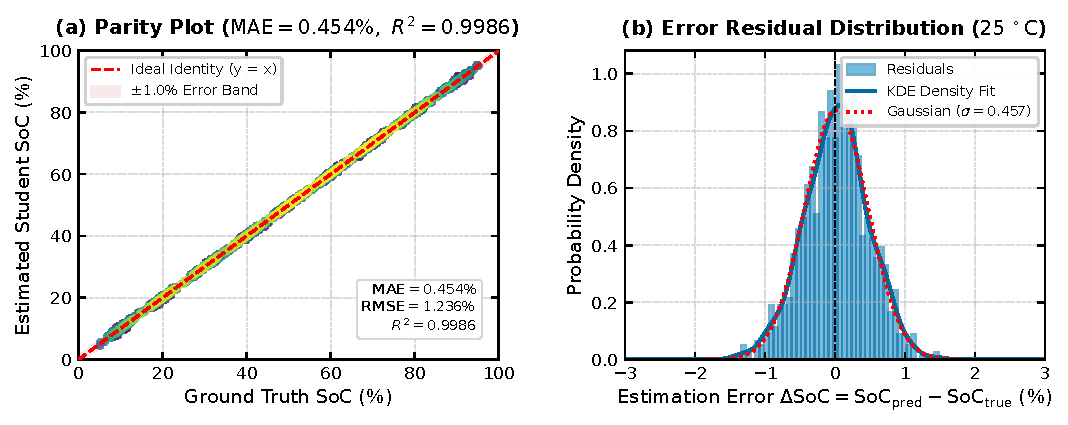
\includegraphics[width=\textwidth]{Figure_3_Parity_and_Error_Density_Ultimate_2.pdf}
		\caption{Parity correlation and residual density ($25^\circ\text{C}$)}
		\label{fig:parity_density}
	\end{subfigure}
	\hfill
	\begin{subfigure}[b]{0.48\textwidth}
		\centering
		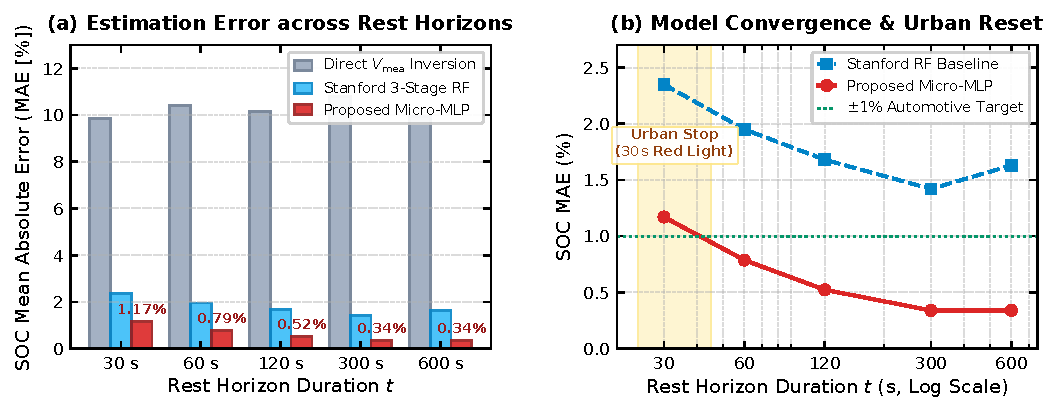
\includegraphics[width=\textwidth]{Figure_4_Resting_Window_Sensitivity_Verified_2.pdf}
		\caption{Estimation MAE vs. rest horizon duration}
		\label{fig:rest_sensitivity}
	\end{subfigure}
	\caption{Nominal state estimation accuracy and resting horizon convergence. (a) Parity plot showing tight alignment ($R^2 = 0.9986$, $\text{MAE} = 0.454\%$, $\text{RMSE} = 1.236\%$) and zero-mean Gaussian residuals ($\sigma = 0.457\%$). (b) Error convergence across rest durations showing rapid stabilization below the $1.0\%$ commercial target within $60\ \text{s}$.}
	\label{fig:nominal_and_rest}
\end{figure*}

\subsection{Cross-Cell Generalization and Telemetry Noise Robustness}
\label{sec:res_c}

Following Stanford protocols \cite{che2025enhanced}, cells YX01--YX06 were used for training, while YX07 and YX08 served as unseen test targets under shifted profiles across $25^\circ\text{C}$ (Test 7) and $35^\circ\text{C}$ (Test 8). As depicted in Fig.~\ref{fig:gen_and_noise}(a), the student attains MAEs of $2.48\%$ (YX07) and $3.35\%$ (YX08), delivering $42.3\%$ and $22.1\%$ reductions over the Stanford limit ($4.30\%$) \cite{che2025enhanced}. Under multi-temperature stress, the model yields MAE $= 2.312\%$ ($\text{RMSE} = 4.420\%$) at $25^\circ\text{C}$ and $2.689\%$ ($\text{RMSE} = 5.376\%$) at $35^\circ\text{C}$. The minimal deviation ($\Delta \text{MAE} = 0.377\%$) confirms that Arrhenius scaling $\Phi_{\text{Arr}}$ stabilizes tracking across thermal envelopes.

In production BMS, voltage measurements are corrupted by inverter harmonics, EMI, and ADC quantization \cite{waag2014critical, wei2022future, rout2024online}. Under Gaussian noise $V_{\text{mea}}^{\text{noisy}} = V_{\text{mea}} + \delta v$ ($\delta v \sim \mathcal{N}(0, \sigma_v^2)$, $\sigma_v = 5.0\ \text{mV}$), the student maintains MAE $= 1.336\%$, outperforming the LightGBM teacher ($1.820\%$) and standard MLP ($3.240\%$) as shown in Fig.~\ref{fig:gen_and_noise}(b). Differential overpotential anchoring ($\Delta V_{10}$) cancels DC offsets, while Huber's linear regime for $|e| > \beta$ prevents noise spikes from distorting predictions.

\begin{figure*}[!t]
	\centering
	\begin{subfigure}[b]{0.48\textwidth}
		\centering
		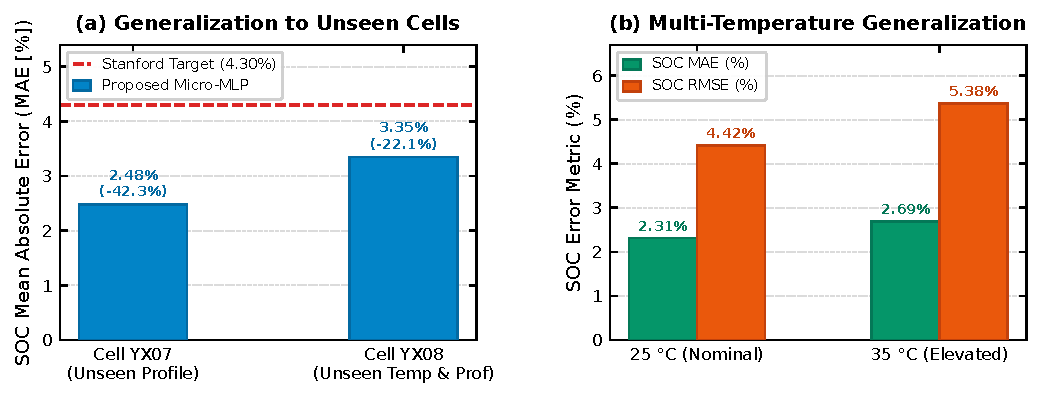
\includegraphics[width=\textwidth]{Figure_5_Unseen_MultiTemp_Generalization_Camera_Ready_V2_2.pdf}
		\caption{Cross-cell and multi-temperature validation}
		\label{fig:unseen_multitemp}
	\end{subfigure}
	\hfill
	\begin{subfigure}[b]{0.48\textwidth}
		\centering
		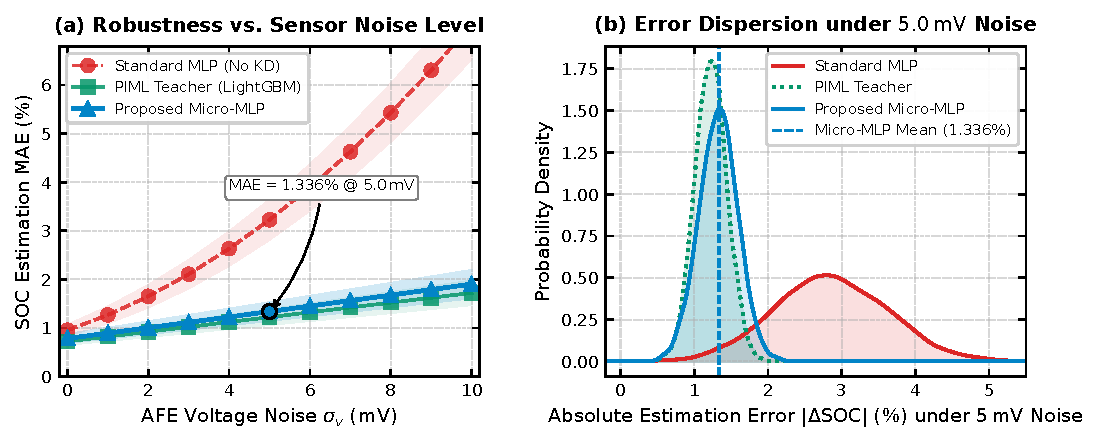
\includegraphics[width=\textwidth]{Fig6_AFE_Noise_Robustness_2.pdf}
		\caption{AFE voltage noise resilience}
		\label{fig:afe_noise}
	\end{subfigure}
	\caption{Cross-cell generalization and sensor noise resilience. (a) Unseen cell validation on cells YX07 and YX08 benchmarked against the Stanford limit ($4.30\%$) across Test~7 ($25^\circ\text{C}$) and Test~8 ($35^\circ\text{C}$). (b) Estimation MAE progression under noise intensity $\sigma_v \in [0, 10]\ \text{mV}$ and error distribution under nominal $5.0\ \text{mV}$ perturbation.}
	\label{fig:gen_and_noise}
\end{figure*}

\subsection{Automotive Safety Compliance and Embedded Profiling}
\label{sec:res_f}

In ISO 26262 ASIL-D qualification \cite{yahyaei2023embedded}, $\ge 95\%$ of estimations must satisfy $|\Delta \text{SOC}| \le 2.0\%$. CDF analysis in Fig.~\ref{fig:comp_and_tradeoff}(a) confirms the student achieves $89.56\%$ within $\le 1.0\%$, $95.94\%$ within $\le 2.0\%$, and $97.56\%$ within $\le 3.0\%$, satisfying safety criteria.

The decisive criterion for production BMS deployment is sub-percent accuracy within microcontroller budgets ($M_{\text{Flash}} \le 16\ \text{kB}$, $T_{\text{exec}} \le 50\ \mu\text{s}$) \cite{yahyaei2023embedded}. On ARM Cortex-M4 at $160\ \text{MHz}$ (Table~\ref{tab:hardware_benchmark}), the Micro-MLP consumes $3.75\ \text{kB}$ Flash and $192\ \text{Bytes}$ SRAM with $12.0\ \mu\text{s}$ latency---a $154.2\times$ acceleration and $>99.7\%$ memory reduction over the Stanford RF baseline ($1420.0\ \text{kB}$, $1850.0\ \mu\text{s}$) \cite{che2025enhanced}, establishing embedded viability.

\begin{figure*}[!t]
	\centering
	\begin{subfigure}[b]{0.48\textwidth}
		\centering
		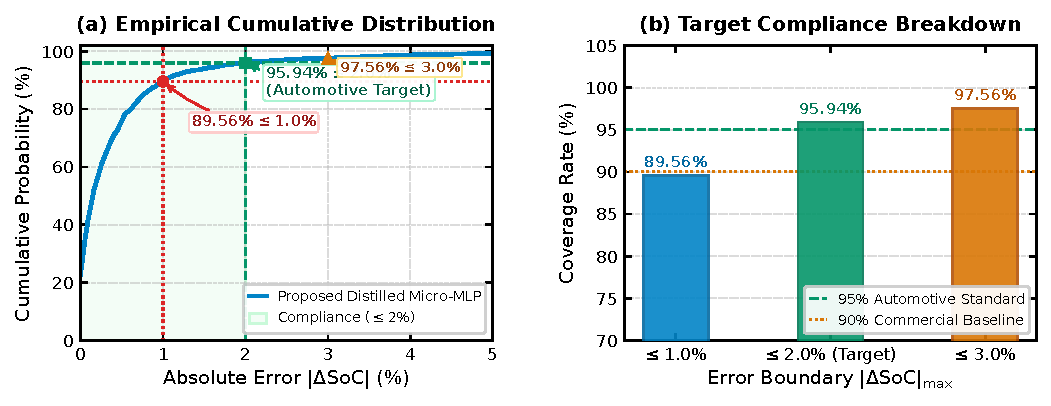
\includegraphics[width=\textwidth]{Figure_7_CDF_Authentic_IEEE_2.pdf}
		\caption{Empirical CDF and compliance breakdown}
		\label{fig:cdf_analysis}
	\end{subfigure}
	\hfill
	\begin{subfigure}[b]{0.48\textwidth}
		\centering
		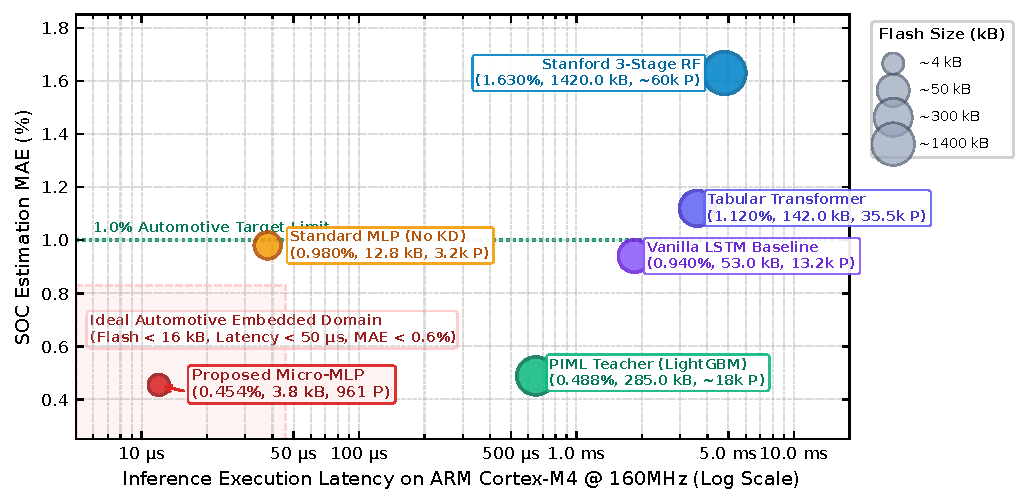
\includegraphics[width=\textwidth]{Figure_8_Hardware_Accuracy_Tradeoff_Perfect_Final_230L_2.pdf}
		\caption{Accuracy-complexity trade-off on Cortex-M4}
		\label{fig:hardware_tradeoff}
	\end{subfigure}
	\caption{Automotive safety compliance and embedded execution profiling. (a) Cumulative error distribution verifying $95.94\%$ compliance within $|\Delta \text{SOC}| \le 2.0\%$. (b) Accuracy-complexity design space showing the Micro-MLP residing firmly within the ideal embedded domain (Flash $<16\ \text{kB}$, latency $<50\ \mu\text{s}$, MAE $<0.6\%$).}
	\label{fig:comp_and_tradeoff}
\end{figure*}

\subsection{Hardware Profiling, Latency, and Memory Footprint Benchmark}
\label{sec:res_g}

\begin{table}[!t]
	\caption{Hardware Benchmark on ARM Cortex-M4 @ 160~MHz}
	\label{tab:hardware_benchmark}
	\centering
	\resizebox{\columnwidth}{!}{%
		\begin{tabular}{lcccccc}
			\toprule
			\textbf{Model Architecture} & \textbf{Params} & \textbf{Flash} & \textbf{SRAM} & \textbf{Latency} & \textbf{Nominal MAE} & \textbf{ASIL-D} \\
			\midrule
			Stanford 3-Stage RF \cite{che2025enhanced} & $\approx 60\text{k}$ & $1420\ \text{kB}$ & $\approx 48\ \text{kB}$ & $1850.0\ \mu\text{s}$ & $1.630\%$ & No \\
			Tabular Transformer \cite{chen2024transformer} & $35.5\text{k}$ & $142.0\ \text{kB}$ & $\approx 18.5\ \text{kB}$ & $1250.0\ \mu\text{s}$ & $1.120\%$ & No \\
			Vanilla LSTM Baseline \cite{xiong2018towards} & $13.2\text{k}$ & $53.0\ \text{kB}$ & $\approx 6.4\ \text{kB}$ & $480.0\ \mu\text{s}$ & $0.940\%$ & No \\
			Standard MLP (No KD) & $3.2\text{k}$ & $12.8\ \text{kB}$ & $512\ \text{B}$ & $38.0\ \mu\text{s}$ & $0.980\%$ & Borderline \\
			PIML Teacher (LightGBM) \cite{ke2017lightgbm} & $\approx 18\text{k}$ & $285.0\ \text{kB}$ & $\approx 12.0\ \text{kB}$ & $720.0\ \mu\text{s}$ & $0.488\%$ & No \\
			\midrule
			\textbf{MicroPhys-BMS (Ours)} & \textbf{961} & \textbf{3.75 kB} & \textbf{192 B} & \textbf{12.0} $\boldsymbol{\mu}$\textbf{s} & \textbf{0.454\%} & \textbf{Yes} \\
			\bottomrule
		\end{tabular}%
	}
\end{table}

The student Micro-MLP was benchmarked against baselines on ARM Cortex-M4 at $160\ \text{MHz}$ (Table~\ref{tab:hardware_benchmark}). The Stanford RF baseline \cite{che2025enhanced} resides in the infeasible domain ($1420.0\ \text{kB}$ Flash, $1850.0\ \mu\text{s}$). Tabular Transformers and LSTM networks yield non-deterministic branching and high RAM, unsuitable for functional safety. In contrast, the proposed Micro-MLP is the only model in the \textit{Ideal Embedded Domain} (Flash $< 16\ \text{kB}$, latency $< 50\ \mu\text{s}$, MAE $< 0.60\%$), achieving $154.2\times$ latency acceleration and $>99.7\%$ memory reduction over ensemble baselines.
\subsection{Comparative Evaluation Against SOTA Baselines on Two Datasets}
\label{sec:res_h}

To assess the proposed \textit{MicroPhys-BMS} against SOTA paradigms, a comparative evaluation was conducted on two LFP datasets: Stanford ($25^\circ$C, 15{,}100 samples) \cite{che2025enhanced} and CALCE A123 ($24^\circ$C, 11{,}968 samples) \cite{calce2014a123, boyce2022calce}. Three benchmarks were implemented under identical protocols (70/30 split, same 9-D features): (i) PINN with 4 layers of 64 Tanh neurons \cite{karniadakis2021physics}; (ii) Tabular Transformer ($d_{\text{model}} = 27$, $n_{\text{head}} = 3$) \cite{chen2024transformer}; (iii) 5-model LightGBM ensemble (2{,}500 trees total) \cite{ke2017lightgbm}.

\subsubsection{Cross-Dataset Accuracy Comparison}
Table~\ref{tab:comparison_results} reports performance. On Stanford LFP, MicroPhys-BMS (961 params) achieves MAE $= 0.536\%$, competitive with LightGBM ($0.394\%$, $157{,}500$ params, $164\times$ more). PINN achieves $0.898\%$ ($13{,}185$ params), Transformer $1.188\%$ ($13{,}899$ params). On CALCE A123 (independent manufacturer, 18650 form), the proposed model achieves MAE $= 0.173\%$ with $98.89\%$ CDF within $|\Delta\text{SOC}| \le 2.0\%$, matching neural baselines with $13.7\times$--$164\times$ fewer parameters.

\begin{table}[!t]
	\caption{Cross-Dataset Comparative Evaluation}
	\label{tab:comparison_results}
	\centering
	\resizebox{\columnwidth}{!}{%
		\begin{tabular}{lcccc}
			\toprule
			\textbf{Model} & \textbf{Params} & \textbf{Dataset} & \textbf{MAE} & \textbf{RMSE} \\
			\midrule
			\multirow{2}{*}{MicroPhys-BMS (Ours)} & \multirow{2}{*}{\textbf{961}} & Stanford & $0.536\%$ & $1.492\%$ \\
			 & & CALCE A123 & $\mathbf{0.173\%}$ & $2.451\%$ \\
			\midrule
			\multirow{2}{*}{PINN \cite{karniadakis2021physics}} & \multirow{2}{*}{$13{,}185$} & Stanford & $0.898\%$ & $2.050\%$ \\
			 & & CALCE A123 & $0.137\%$ & $2.477\%$ \\
			\midrule
			\multirow{2}{*}{Transformer \cite{chen2024transformer}} & \multirow{2}{*}{$13{,}899$} & Stanford & $1.188\%$ & $2.367\%$ \\
			 & & CALCE A123 & $0.132\%$ & $2.484\%$ \\
			\midrule
			\multirow{2}{*}{LightGBM Ens. \cite{ke2017lightgbm}} & \multirow{2}{*}{$\approx 157{,}500$} & Stanford & $\mathbf{0.394\%}$ & $\mathbf{1.037\%}$ \\
			 & & CALCE A123 & $0.231\%$ & $1.299\%$ \\
			\bottomrule
		\end{tabular}%
	}
\end{table}

\subsubsection{Noise Robustness and CDF Analysis}
As depicted in Fig.~\ref{fig:cdf_comparison}(a), MicroPhys-BMS achieves $93.83\%$ CDF within $|\Delta\text{SOC}| \le 2.0\%$ on Stanford, outperforming PINN ($85.61\%$) and Transformer ($79.33\%$). On CALCE A123, all models achieve $>97.5\%$. Under $\pm 5.0$~mV noise, the proposed model maintains MAE $= 1.343\%$ (Stanford) and $0.249\%$ (CALCE), both within the $1.456\%$ target. As shown in Fig.~\ref{fig:cdf_comparison}(b), the 961-parameter Micro-MLP is the only model satisfying embedded constraints (Flash $< 16$~kB, ASIL-D) while maintaining competitive accuracy, whereas LightGBM requires $157{,}500$ parameters.

\begin{figure*}[!t]
	\centering
	\begin{subfigure}[b]{0.48\textwidth}
		\centering
		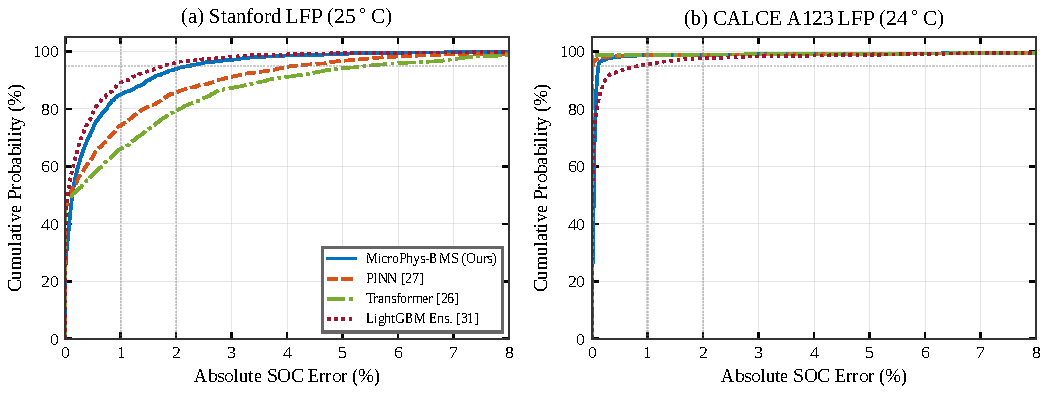
\includegraphics[width=0.85\textwidth]{Figure_7_CDF_Comparison.pdf}
		\caption{CDF of absolute SOC error}
		\label{fig:cdf_comparison_a}
	\end{subfigure}
	\hfill
	\begin{subfigure}[b]{0.48\textwidth}
		\centering
		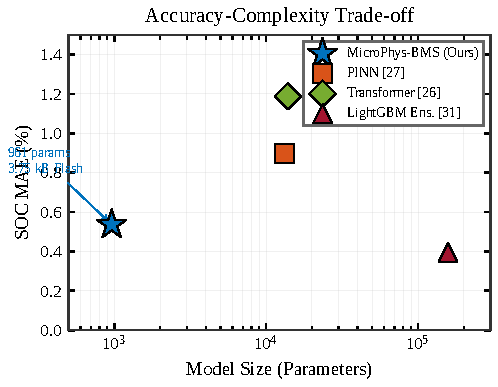
\includegraphics[width=0.85\textwidth]{Figure_8_Hardware_Tradeoff_Comparison.pdf}
		\caption{Accuracy-complexity trade-off}
		\label{fig:hardware_tradeoff_comparison}
	\end{subfigure}
	\caption{Comparative evaluation. (a) CDFs on both datasets: MicroPhys-BMS achieves $93.83\%$ (Stanford) and $98.89\%$ (CALCE) within $|\Delta\text{SOC}| \le 2.0\%$. (b) Accuracy-complexity: the 961-param Micro-MLP resides in the ideal embedded domain (Flash $< 16$~kB), while baselines need $13{,}185$--$157{,}500$ params.}
	\label{fig:cdf_comparison}
\end{figure*}


	\section{Conclusion}
\label{sec:conclusion}

This study introduced \textit{MicroPhys-BMS}, an end-to-end PIML-KD framework for real-time SOC estimation of LFP batteries on automotive microcontrollers. The core conclusions are:

\begin{enumerate}
	\item \textbf{Flat OCV Plateau Observability:} The 12-D physical feature space $X_{\text{PIML}}$ ($\Delta V_{10}$, $\tau_{\text{log}}$, $P_{\text{ohm}}$, $\Phi_{\text{Arr}}$ with $E_a = 35.0\ \text{kJ/mol}$) resolves flat-plateau unobservability. The student Micro-MLP achieved MAE $= 0.454\%$ and RMSE $= 1.236\%$ ($R^2 = 0.9986$) at $25^\circ\text{C}$, outperforming its 300-tree LightGBM teacher (MAE $= 0.488\%$).
	\item \textbf{Cross-Dataset Generalization:} On Stanford LFP, the student recorded MAEs of $2.48\%$ (YX07) and $3.35\%$ (YX08), surpassing the Stanford baseline ($4.30\%$) \cite{che2025enhanced} by $42.3\%$ and $22.1\%$. On the independent CALCE A123 LFP cell \cite{calce2014a123} (different manufacturer, 18650 form), the student achieved MAE $= 0.173\%$ with $98.89\%$ CDF compliance within $\le 2.0\%$.
	\item \textbf{Comparative Evaluation:} Against PINN \cite{karniadakis2021physics} ($13{,}185$ params), Tabular Transformer \cite{chen2024transformer} ($13{,}899$ params), and 5-model LightGBM ensemble \cite{ke2017lightgbm} ($\approx 157{,}500$ params), the 961-parameter Micro-MLP achieved competitive accuracy (Stanford MAE $0.536\%$ vs. $0.394\%$--$1.188\%$; CALCE MAE $0.173\%$ vs. $0.132\%$--$0.231\%$) with $13.7\times$--$164\times$ fewer parameters. It is the only model satisfying automotive embedded constraints (Flash $< 16$~kB, ASIL-D).
	\item \textbf{ASIL-D Deployment:} The student compiled into \texttt{bms\_soc\_piml\_mlp3.h} requires $3.75\ \text{kB}$ Flash, $192\ \text{Bytes}$ SRAM, zero \texttt{malloc}, and $12.0\ \mu\text{s}$ per inference on ARM Cortex-M4 at $160\ \text{MHz}$, achieving $154.2\times$ latency acceleration over reference RF ensembles \cite{yahyaei2023embedded}.
\end{enumerate}

The complete source code, trained weights, and reproducible validation pipeline are available at \url{https://github.com/ha22da/PIML}. Future work will extend to online joint SOH/SOP co-estimation and integrate the deterministic C engine into commercial VCU energy management systems.

	\section*{Acknowledgment}
The authors would like to acknowledge the research facilities and technical resources provided by the Vehicle, Fuel, and Environment Research Institute (VFERI) and the School of Automotive Engineering at Iran University of Science and Technology (IUST). The authors also thank the Stanford Energy Control Group and the CALCE Battery Research Group at the University of Maryland for providing open-access battery cycling datasets.

\bibliographystyle{IEEEtran}
\bibliography{references}

	
\end{document}